\chapter{Worldsheets, Wick Rotation, and Channel Duality}

\lectureoverview{A particle traces a worldline; a string sweeps out a
worldsheet.  Quantizing either object requires a sum over histories, but the
Lorentzian sum is oscillatory and difficult to define.  Turning worldsheet
time into an imaginary coordinate gives a Euclidean theory governed by the
Laplace equation.  Its conformal symmetry then turns the slit surface of a
four-string interaction into a disc with four boundary insertions, where the
symmetry between direct and crossed channels becomes visible.}

\section{From a Worldline to a Sum over Histories}

Begin with a free particle.  In nonrelativistic mechanics its position is a
function \(\mathbf x(t)\), and, with the mass set to one, its action is
\begin{equation}
  S_{\mathrm{NR}}[\mathbf x]
  =\frac12\int_{t_1}^{t_2}\dot{\mathbf x}^{\,2}\,dt.
  \label{eq:l07-nr-action}
\end{equation}
For a relativistic description it is more natural to place time and space in
one vector, \(X^\mu(\tau)\), parameterized along the trajectory by \(\tau\).
The corresponding quadratic expression is
\begin{equation}
  S_{\mathrm{rel}}[X]
  =\frac12\int_{\tau_1}^{\tau_2}
  \frac{dX^\mu}{d\tau}\frac{dX_\mu}{d\tau}\,d\tau.
  \label{eq:l07-rel-action}
\end{equation}
The upper and lower indices encode the Lorentzian sign difference between
time and space.
\editorialnote{The quadratic relativistic action is being used in a fixed
worldline parameterization.  The manifestly reparameterization-invariant
alternative is proportional to proper length, which is mentioned later in
the lecture.}

\begin{figure}[H]
  \centering
  
\includegraphics[width=0.72\textwidth]{lecture_07_figure_01.png}
  \caption{The nonrelativistic action and its relativistic quadratic
  counterpart written together on the board.}
  \lectureframe{00:03:35}
  \label{fig:l07-particle-actions}
\end{figure}

Classically, one fixes the endpoints and varies the path.  A free particle
then follows a straight worldline with constant velocity.  Quantum mechanics
asks a different question.  It does not select one trajectory between the
endpoints; it asks for the amplitude to begin at one point and be detected at
the other.  Every intervening path contributes a phase,
\begin{equation}
  K(2,1)=\int_{X(1)}^{X(2)}\!\mathcal D X\,
  e^{iS[X]}.
  \label{eq:l07-feynman-integral}
\end{equation}
The functional integral is an integral over an infinite-dimensional space of
paths, not the ordinary integral already appearing inside the action.

\begin{figure}[H]
  \centering
  
\includegraphics[width=0.72\textwidth]{lecture_07_figure_02.png}
  \caption{A representative path and the phase assigned to it before the
  sum over all trajectories is taken.}
  \lectureframe{00:06:21}
  \label{fig:l07-path-integral-board}
\end{figure}

In relativistic language this point-to-point amplitude is a propagator.  For
an interaction, several worldline segments meet.  Their actions are added,
the meeting points are integrated over, and diagrams with the required
external particles are summed.  Thus the familiar Feynman-diagram expansion
is already implicit in the instruction to sum over histories.

The symbol \(S\) will denote an action here.  It is unrelated both to entropy
and to the Mandelstam variable \(s\) used near the end of the lecture.  The
shared notation is traditional rather than illuminating.

\section{Turning Time Sideways}

There is an immediate problem with \eqref{eq:l07-feynman-integral}.  Every
factor \(e^{iS}\) has magnitude one.  A wildly oscillating trajectory and the
classical straight line therefore enter with equal absolute weight; only
their phases differ.  Destructive interference recovers classical behavior,
but it does not make the formal integral an ordinary convergent object.

Introduce a new parameter \(s\) through
\begin{equation}
  \tau=\alpha s,
  \qquad
  d\tau=\alpha\,ds,
  \qquad
  \frac{dX}{d\tau}=\frac{1}{\alpha}\frac{dX}{ds}.
\end{equation}
Then the quadratic action rescales as
\begin{equation}
  \frac12\int d\tau
  \left(\frac{dX}{d\tau}\right)^2
  =
  \frac{1}{2\alpha}\int ds
  \left(\frac{dX}{ds}\right)^2.
  \label{eq:l07-rescaled-action}
\end{equation}
Choosing the contour corresponding to \(\alpha=-i\) changes the oscillatory
weight into
\begin{equation}
  e^{iS}
  \longrightarrow
  \exp\!\left[-\frac12\int ds
  \left(\frac{dX}{ds}\right)^2\right]
  =e^{-S_E}.
  \label{eq:l07-euclidean-particle}
\end{equation}

\begin{figure}[H]
  \centering
  
\includegraphics[width=0.66\textwidth]{lecture_07_figure_03.png}
  \caption{The Euclidean particle weight after the imaginary-time
  substitution; the exponent is real and nonpositive.}
  \lectureframe{00:16:20}
  \label{fig:l07-particle-wick}
\end{figure}

A path that runs far away and returns, or wiggles rapidly without traveling
far, has a large positive \(S_E\) and is exponentially suppressed.  The
result is a Wiener-type integral, for which a serious convergence theory
exists.  The endpoints inherited from real \(\tau\) lie on an imaginary
\(s\)-contour.  In practice one evaluates the Euclidean object in its
convergent domain and analytically continues the answer back to the physical
Lorentzian variables.  This operation is the Wick rotation: time has been
turned sideways for the calculation, not discarded.

\section{From Worldlines to Worldsheets}

A point particle has a worldline.  An open string sweeps out a ribbon, and a
closed string sweeps out a tube.  Coordinates \((\sigma,\tau)\) label points
on this two-dimensional worldsheet, while
\begin{equation}
  X^\mu=X^\mu(\sigma,\tau)
  \label{eq:l07-embedding}
\end{equation}
gives the spacetime position of the labeled point.  Knowing all the functions
\(X^\mu\) specifies the complete history of the string.

The quadratic Lorentzian worldsheet action has the same kinetic-minus-
potential structure as an ordinary vibrating string:
\begin{equation}
  S_{\mathrm{ws}}[X]
  =\frac{T_s}{2}\int d\tau\,d\sigma\,
  \left[
    \partial_\tau X^\mu\partial_\tau X_\mu
    -
    \partial_\sigma X^\mu\partial_\sigma X_\mu
  \right].
  \label{eq:l07-lorentzian-worldsheet}
\end{equation}
The overall tension \(T_s\) fixes the scale; the lecture suppresses it while
concentrating on the derivative structure.

\begin{figure}[H]
  \centering
  
\includegraphics[width=0.72\textwidth]{lecture_07_figure_04.png}
  \caption{The Lorentzian worldsheet action for
  \(X^\mu(\sigma,\tau)\), with its kinetic-minus-potential sign.}
  \lectureframe{00:24:26}
  \label{fig:l07-worldsheet-action}
\end{figure}

The string amplitude is obtained by exponentiating this action and summing
over all surfaces connecting prescribed initial and final string
configurations:
\begin{equation}
  \mathcal A=\int\mathcal D X\,e^{iS_{\mathrm{ws}}[X]}.
  \label{eq:l07-surface-integral}
\end{equation}
The same rule handles two strings becoming two, two becoming three, or any
other allowed external configuration.  Different worldsheet topologies also
belong to the sum.  Adding holes is the string counterpart of adding loop
orders in a point-particle diagram expansion.

\begin{figure}[H]
  \centering
  
\includegraphics[width=0.66\textwidth]{lecture_07_figure_05.png}
  \caption{A surface connecting several external strings, with a hole
  representing a different worldsheet topology.}
  \lectureframe{00:27:14}
  \label{fig:l07-surface-topology}
\end{figure}

\begin{classroomqa}
\audiencequestion{For a point electron, does the \(\sigma\)-derivative simply
vanish? \lecturetimestamp{00:27:56}}
\lecturerresponse{A point particle has no \(\sigma\) coordinate in the first
place.  Nevertheless the pictures are connected: when external states are
light compared with the string scale and process energies are low, string
amplitudes reproduce ordinary point-particle Feynman diagrams.  That limit is
more than setting one derivative to zero.}
\end{classroomqa}

The surface integral has the same convergence problem as the path integral.
After Wick-rotating worldsheet time, its stable Euclidean form is
\begin{equation}
  S_{E,\mathrm{ws}}[X]
  =\frac{T_s}{2}\int d\tau\,d\sigma\,
  \left[
    \partial_\tau X^\mu\partial_\tau X_\mu
    +
    \partial_\sigma X^\mu\partial_\sigma X_\mu
  \right],
  \qquad
  \mathcal A_E=\int\mathcal D X\,e^{-S_{E,\mathrm{ws}}}.
  \label{eq:l07-euclidean-worldsheet}
\end{equation}
Both derivatives now enter with the same positive sign.  A violently
vibrating or greatly stretched surface has large Euclidean action and is
suppressed.

\begin{figure}[H]
  \centering
  
\includegraphics[width=0.72\textwidth]{lecture_07_figure_06.png}
  \caption{The positive Euclidean worldsheet density after
  \(\tau\) is rotated to imaginary time.}
  \lectureframe{00:34:29}
  \label{fig:l07-worldsheet-wick}
\end{figure}

There is also a geometrically direct formulation.  A relativistic particle
may be assigned an action proportional to the proper length of its path; a
string may be assigned an action proportional to the spacetime area of its
worldsheet.  The latter is the Nambu--Goto action.  The quadratic worldsheet
form used here is conventionally called the Polyakov form and is much easier
for the present calculation.
\editorialnote{The lecture includes a humorous discussion of historical
naming and also mentions the related Liouville action and Dirichlet boundary
conditions.  No priority claim is needed for the derivation: only the
equivalence of the area and auxiliary-metric formulations is used.}

\section{The Euclidean Equation of Motion}

The coordinates \(\sigma\) and \(\tau\) are only labels on the sheet.  The
next question is therefore unavoidable: which relabelings leave the theory
unchanged?  The answer is easiest to see from the equation of motion.
Varying \eqref{eq:l07-euclidean-worldsheet} gives, component by component,
\begin{equation}
  \partial_\tau^2X^\mu+\partial_\sigma^2X^\mu=0.
  \label{eq:l07-laplace}
\end{equation}
Before Wick rotation the relative sign is negative and this is a wave
equation.  In Euclidean signature both signs are positive, so it is the
two-dimensional Laplace equation.

\begin{classroomqa}
\audiencequestion{Is this the equation of a vibrating drum?
\lecturetimestamp{00:41:50}}
\lecturerresponse{It is closely related, but a vibrating drum also carries a
real time coordinate and therefore obeys a wave equation.  The equation here
is Euclidean Laplace's equation.  Electrostatic potential in a charge-free
region supplies a more direct familiar example.}
\end{classroomqa}

\begin{classroomqa}
\audiencequestion{The action contains first derivatives.  Why does its
equation contain second derivatives? \lecturetimestamp{00:42:44}}
\lecturerresponse{Varying a term quadratic in a first derivative and
integrating by parts moves one derivative onto that first derivative.  It is
the field-theory version of \(\dot x^{\,2}\) in an action producing
\(\ddot x\) in the equation of motion.}
\end{classroomqa}

\begin{figure}[H]
  \centering
  
\includegraphics[width=0.68\textwidth]{lecture_07_figure_07.png}
  \caption{The plus-sign Laplace equation and the first discrete line used
  to interpret its second derivatives.}
  \lectureframe{00:43:30}
  \label{fig:l07-laplace-board}
\end{figure}

To see the geometry, first discretize one coordinate with spacing
\(\epsilon\).  A first derivative is a neighboring difference, while a
second derivative is a difference of neighboring differences:
\begin{equation}
  \frac{d^2X}{ds^2}\bigg|_{2}
  \longrightarrow
  \frac{X(3)-2X(2)+X(1)}{\epsilon^2}.
  \label{eq:l07-second-difference}
\end{equation}

\begin{figure}[H]
  \centering
  
\includegraphics[width=0.72\textwidth]{lecture_07_figure_08.png}
  \caption{The numbered line, small lattice patch, and finite-difference
  expansion of a second derivative.}
  \lectureframe{00:45:51}
  \label{fig:l07-finite-difference-board}
\end{figure}

Now discretize the \((\sigma,\tau)\)-plane.  Label four nearest neighbors of
a central point \(5\) by \(1,2,3,4\).  Equation
\eqref{eq:l07-laplace} becomes
\begin{equation}
  X(1)+X(2)+X(3)+X(4)-4X(5)=0,
\end{equation}
or
\begin{equation}
  X(5)=\frac14\bigl[X(1)+X(2)+X(3)+X(4)\bigr].
  \label{eq:l07-mean-value}
\end{equation}

\begin{figure}[H]
  \centering
  
\includegraphics[width=0.72\textwidth]{lecture_07_figure_09.png}
  \caption{The completed two-dimensional finite-difference equation: the
  central value equals the average of its four neighbors.}
  \lectureframe{00:48:26}
  \label{fig:l07-mean-value-board}
\end{figure}

This mean-value property holds for an infinitesimal square in any
orientation.  It is the local geometric content of the Laplace equation and
the bridge to conformal symmetry.

\section{Conformal Coordinates}

Consider a change from \((\sigma,\tau)\) to
\((\sigma',\tau')\).  A general deformation sends a small square to an
arbitrary quadrilateral.  The special transformations relevant here send
every infinitesimal square to another infinitesimal square, possibly rotated
and rescaled.  Equivalently, they preserve the angles at which curves meet.
These are conformal transformations.

\begin{figure}[H]
  \centering
  
\includegraphics[width=0.68\textwidth]{lecture_07_figure_10.png}
  \caption{A local square mapped to another small figure while its angles
  are tested for conformal preservation.}
  \lectureframe{00:53:25}
  \label{fig:l07-conformal-board}
\end{figure}

\begin{classroomqa}
\audiencequestion{If angles are preserved, is the transformation basically
only a rotation? \lecturetimestamp{00:53:31}}
\lecturerresponse{Only locally, and even there a common scale change is also
allowed.  The local rotation and scale factor may vary from point to point,
so the coordinate grid can bend, expand in one region, and contract in
another while preserving infinitesimal shapes.}
\end{classroomqa}

An angle-preserving map need not preserve size.  If size were also fixed
everywhere, the possibilities would collapse to the much smaller rigid class
of translations and rotations.  Conformal maps instead preserve local shape.
This is why a map projection can keep the shape of a small island while
greatly distorting its area.

\begin{classroomqa}
\audiencequestion{Is a conformal mapping equivalent to saying that the
coordinate system is flat? \lecturetimestamp{00:55:35}}
\lecturerresponse{No.  Flatness and conformality are different statements.
A conformal map may use curved coordinate lines; what it preserves is the
angle between intersecting curves.  A Mercator-type map projection is a
familiar example of local shape preservation with substantial scale
distortion.}
\end{classroomqa}

In two dimensions the required transformations are generated locally by
analytic functions of a complex coordinate
\begin{equation}
  z=\sigma+i\tau.
\end{equation}
Finite boundaries can change appearance dramatically.  A square region may
be mapped to a smooth region, with the original corners sent to ordinary
points on the new boundary rather than to its visually prominent points.
There is no contradiction: conformality is a local interior condition, and
the map preserves infinitesimal angles wherever it is regular.

\begin{classroomqa}
\audiencequestion{Is this coordinate freedom the reason the earlier
join--split diagram could be chosen symmetrically?
\lecturetimestamp{00:56:32}}
\lecturerresponse{Yes.  The same conformal freedom that preserves the
worldsheet equations lets us replace the awkward interaction strip by a
more symmetric domain.  The remaining freedom does not remove the physical
join--split parameter; it repackages that parameter as the relative position
of boundary insertions.}
\end{classroomqa}

\section{The Slit Sheet and the Disc}

Return to four-string scattering.  Two open strings enter, their endpoints
join, the combined string propagates, and it later splits.  Drawn as a flat
worldsheet, the process is an infinite strip slit from each end.  The
separation \(\tau_0\) between the tips of the slits is the lifetime of the
intermediate string, and the amplitude integrates over it.

\begin{figure}[H]
  \centering
  
\includegraphics[width=0.72\textwidth]{lecture_07_figure_11.png}
  \caption{The doubly slit strip representing two open strings joining,
  propagating together, and splitting again.}
  \lectureframe{01:00:20}
  \label{fig:l07-slit-strip}
\end{figure}

After Euclideanization, the embedding fields on this region satisfy the
Laplace equation.  Conformal invariance therefore permits the slit strip to
be mapped to a disc.  One way to see the topology is to foliate the disc by
concentric circles and continuously deform those closed curves until they
fill the slit region.  The ends at infinity become exceptional boundary
points under the map.

\begin{figure}[H]
  \centering
  
\includegraphics[width=0.72\textwidth]{lecture_07_figure_12.png}
  \medskip

  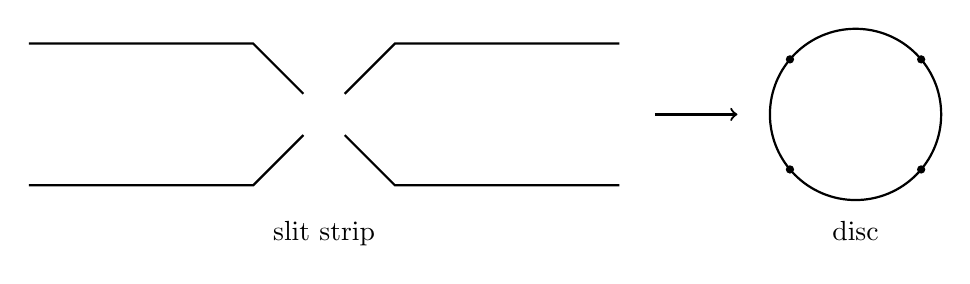
\begin{tikzpicture}[x=0.75cm,y=0.75cm]
    \draw[thick] (-5,1.2) -- (-1.2,1.2) -- (-0.35,0.35);
    \draw[thick] (-5,-1.2) -- (-1.2,-1.2) -- (-0.35,-0.35);
    \draw[thick] (0.35,0.35) -- (1.2,1.2) -- (5,1.2);
    \draw[thick] (0.35,-0.35) -- (1.2,-1.2) -- (5,-1.2);
    \draw[->,thick] (5.6,0) -- (7.0,0);
    \draw[thick] (9.0,0) circle (1.45);
    \foreach \a in {40,140,220,320} \fill (9.0,0) ++(\a:1.45) circle (1.5pt);
    \node[below] at (0,-1.65) {slit strip};
    \node[below] at (9.0,-1.65) {disc};
  \end{tikzpicture}
  \caption{The board's level-curve comparison and a clean schematic of the
  conformal map from the slit strip to a disc.  The four external ends become
  four special boundary points.}
  \lectureframe{01:04:46}
  \label{fig:l07-strip-to-disc}
\end{figure}

The external states are not lost in this change of coordinates.  Momentum,
particle type, and oscillator level must be inserted at the four exceptional
points.  The formal objects carrying that information are vertex operators.
Their detailed construction is deferred, but their role is already clear:
they turn an otherwise homogeneous worldsheet path integral into a specified
scattering experiment.

After using conformal transformations of the disc to move three boundary
points to convenient reference positions, one real relative position
remains.  It may be represented by the cross-ratio of the four ordered
boundary points.  This is the disc version of the old lifetime \(\tau_0\).

\begin{figure}[H]
  \centering
  
\includegraphics[width=0.62\textwidth]{lecture_07_figure_13.png}
  \caption{Four insertion points on the boundary of the disc.  Conformal
  freedom removes all but one real modulus of their ordered configuration.}
  \lectureframe{01:10:55}
  \label{fig:l07-four-points}
\end{figure}

The lifetime integral has therefore not disappeared.  It has become an
integral over that remaining modulus.  With a conventional coordinate
\(0<z<1\), the four-point open-string integral takes the same form found in
the preceding lecture,
\begin{equation}
  \mathcal A(s,t)\propto
  \int_0^1 z^{-s-1}(1-z)^{-t-1}\,dz.
  \label{eq:l07-modulus-integral}
\end{equation}

\section{Two Limits of One Surface}

At one end of moduli space, the two insertion points associated with the
incoming pair approach one another.  In the slit-strip coordinates this is a
long interval between joining and splitting: a direct-channel intermediate
string propagates for a long time.  At the other end, a different neighboring
pair approaches.  The same surface is then naturally read as a crossed-
channel exchange.  These descriptions look unrelated on the strip but are
neighboring boundary limits of one disc integral.

Returning to the mostly-plus convention of the previous lecture,
\begin{equation}
  -s=(k_1+k_2)^2,
  \qquad
  -t=(k_1+k_3)^2.
  \label{eq:l07-mandelstam}
\end{equation}
The direct limit organizes poles in \(s\); the crossed limit organizes poles
in \(t\).
\editorialnote{Near the end of the lecture the board uses a shorthand sign
for the Mandelstam invariants while also identifying \(s\) with positive
center-of-mass energy squared.  Equation \eqref{eq:l07-mandelstam} keeps the
mostly-plus convention established in Lecture 6.}

\begin{figure}[H]
  \centering
  
\includegraphics[width=0.62\textwidth]{lecture_07_figure_14.png}
  \caption{The two channel diagrams: long propagation in one orientation
  and exchange in the crossed orientation.}
  \lectureframe{01:19:27}
  \label{fig:l07-channel-diagrams}
\end{figure}

\begin{figure}[H]
  \centering
  
\includegraphics[width=0.72\textwidth]{lecture_07_figure_15.png}
  \caption{The board returns to the \(s\)- and \(t\)-channel momentum
  pairings while comparing the two limits of the disc modulus.}
  \lectureframe{01:19:40}
  \label{fig:l07-st-board}
\end{figure}

One analytic object therefore supplies both expansions:
\begin{equation}
  \mathcal A(s,t)=\mathcal A(t,s).
\end{equation}
This is channel duality.  In the original resonance language it appeared
miraculous that a sum over direct-channel states could also encode crossed-
channel exchange.  On the Euclidean worldsheet, conformal symmetry explains
why the two descriptions belong to the same surface.  Historically this
interpretation followed the 1969 discovery of the Veneziano amplitude very
quickly.

\begin{classroomqa}
\audiencequestion{Is there a slit-strip picture corresponding to the crossed
orientation as well? \lecturetimestamp{01:20:49}}
\lecturerresponse{Yes, but the direction called time must be chosen
differently.  The same Euclidean surface can be sliced so that another pair
of external ends lies in the remote past and future.  That alternative
slicing is precisely why a single worldsheet admits more than one channel
interpretation.}
\end{classroomqa}

\begin{classroomqa}
\audiencequestion{Is the time for which the strings remain joined determined
by the coupling constant? \lecturetimestamp{01:21:39}}
\lecturerresponse{No fixed lifetime is selected.  The lifetime is an
integration variable and every value contributes.  The coupling controls the
weight for joining and splitting---equivalently, the decay strength---and
enters multiplicatively in the amplitude; it does not replace the modulus
integral.}
\end{classroomqa}
